\chapter{Introdução}
Tendo em vista a necessidade de aspiração em piscinas e a crescente onda de automação residencial, observou-se a oportunidade de produzir um equipamento para realizar tal tarefa automática de piscinas (Kanno et al, 2014).

Considerando o alto custo de aquisição de equipamentos modernos, internacionais e a grande demanda por serviços de higienização de piscinas, e o fato de que no Brasil não há empresas que desenvolvam este produto (há apenas revendedoras), o desenvolvimento do Clean Pool Robot permitirá a aplicação do conceito de automação a ambientes residenciais e a redução dos gastos com a contratação de um serviço terceirizado. As principais vantagens na utilização do Clean Pool Robot são:

\begin{itemize}
\item Retirar detritos do fundo da piscina que não foram alcançados por outros meios;
\item Mover a água ao passo que limpa as superfícies, melhorando a sua circulação;
\item Produzir um produto nacional que possui valor de mercado mais acessível.
\end{itemize}

Em uma pesquisa realizada pela equipe, verificou-se que a massa dos robôs que limpam piscinas variam de 8 Kg até 25 Kg e custam entre R\$ 2.000,00 e R\$ 16.000,00. O clean Pool Robot tem massa de aproximadamente 10kg e custará proximo de R\$ 7.000,00, nem o mais caro e nem o mais barato. Para a escolha de um limpador de piscinas automaitico pequenas diferenças de especificação devem ser consideradas no momento da aquisição do aparelho, como por exemplo, ciclo de limpeza e taxa de filtragem. O ciclo de limpeza determina o intervalo de tempo em que o robô trabalha antes de se desligar automaticamente e a taxa de filtragem é determinada pela quantidade de água filtrada em uma hora, que é expressa em litros por hora (LPH). No caso do CPR tem um ciclo de limpeza de 5h, tempo necessario para limpar uma piscina curta (semiolimpica).

Este projeto lida basicamente com um corpo imerso em um líquido, deste modo o corpo estará essencialmente sob ação de duas forças: empuxo e peso.  Empuxo ocorre quando um corpo imerso na água parece ter se tornado mais leve devido a uma força, exercida pelo líquido sobre o corpo, vertical e para cima, que alivia o peso do corpo. Já o peso é devido à interação com o campo gravitacional da Terra.

Quando um corpo está totalmente imerso em um líquido, podemos ter as seguintes situações: 

\begin{itemize}
\item Se ele permanecer parado no ponto onde foi colocado, a intensidade da força de empuxo é igual à intensidade da força peso;
\item Se ele afundar, a intensidade da força de empuxo é menor do que a intensidade da força peso;
\item Se ele for levado para a superfície, à intensidade da força de empuxo é maior do que a intensidade da força peso.
\end{itemize}

Como o robô realiza a limpeza do fundo da piscina, este deve estar afundado, ou seja, a intensidade da força de empuxo deverá ser menor do que a intensidade da força peso.

\section{Objetivos do Projeto}
Construir um robô capaz de realizar a remoção de sujeiras depositadas no fundo de piscinas por meio da aspiração e filtragem das impurezas. O objetivo específico deste relatório é apresentar:

\begin{itemize}
\item O projeto de solução, modelagem, cálculos matemáticos e; 
\item As simulações; 
\item A Prototipagem das partes do robô e da solução.
\end{itemize}

\section{Estrutura do Relatório}
A organização do projeto foi dividido em dois grupos: o grupo de estrutura, design e o grupo de lógica. Ambos os grupos se relacionam e tem trabalhado em conjunto. O diagrama abaixo apresenta a interação entre os grupos e as diversas engenharias que os compõem.
\par
  \begin{figure}[h]
    \centering
    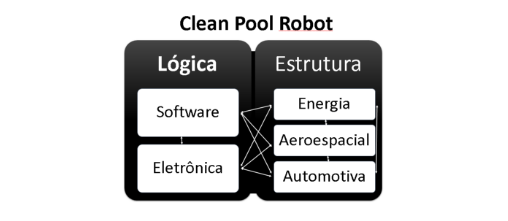
\includegraphics[width=0.8\textwidth]{figures/technical-div-project.png}
    \caption{Divisão técnica do projeto em dois segmentos.}
    \label{fig:technical-div-project}
  \end{figure}
  \FloatBarrier
\par
Apesar da divisão em duas grandes equipes, os membros interagiram de forma a preencher os requisitos e parâmetros solicitados por meio de documentos compartilhados via Google drive, ou por mensagens em grupos de conversa privados, utilizando-se do WhatsApp.

Nos próximos itens do relatório estão a Visão geral no nosso produto, onde apresentamos o seu design, os sistemas que o compõem, os indicadores e a estimativa de custo. Em seguida temos o dimensionamento de cada componente. Por fim temos a montagen do prototipo e os testes realizados no mesmo.

\chapter{O \textit{Clean Pool Robot}}
\section{Visão Geral}
O Clean Pool Robot é equipamento que visa auxiliar a limpeza de grandes piscinas, como os modelos semi-olimpicos. O robô faz a aspiração e filtragem das impurezas presentes no fundo da piscina, removendo as algas e folhas e auxiliando na circulação da água. O mecanismo do mesmo será composto por dois métodos para que o fundo da piscina possa ser aspirado: o primeiro baseia-se na escovação do chão e o segundo a sucção das impurezas desprendidas do piso da piscina.

O primeiro método tem foco nas escovas que estão situadas na parte inferior do robô. As escovas realizam movimentos giratórios fazendo com que suas cerdas entrem em contato com o chão retirando  impurezas, como por exemplo: algas e grãos de terra.

Após a escovação, é realizado outro método, a sucção das impurezas desprendidas do piso da piscina  além de outras impurezas que estiverem próximas à área de atuação do robô, por exemplo: pequenos ramos e folhas. Por meio de uma bomba, a água é sugada por uma abertura situada na parte inferior e passa por um filtro. As impurezas menores ficam retidas no filtro. Por meio de um sistema de expulsão de água, esta sairá a uma velocidade muito superior à velocidade de entrada no início do processo, ajudando na movimentação do robô.

Com o término da limpeza na piscina, haverá a necessidade dos filtros serem limpos para retirada das impurezas colhidas na aspiração da água. Assim, após cada utilização o usuário deverá limpar os filtros internos do robô Clean Pool.

O produto desenvolvido será responsável apenas pela retirada da sujeira decantada no fundo da piscina, ou seja, o Clean Pool Robot não limpará as paredes ou superfície da piscina. Além disso, as piscinas ideais para a operação do Robot são as retangulares, sem inclinações e azulejadas. É ideal também que o robô seja lançado na piscina no meio da largura maior, evitando que o fio fique totalmente esticado quando o robô estiver na quina oposta do lançamento.  

\section{O \textit{Design}}
A figura abaixo mostra o Clean Pool Robot projetado no software Catia. O modelo apresenta dois rolos de limpeza, localizados na parte frontal e traseira do robô, um duto, na parte superior para a saída da água filtrada e também funciona como propulsão e direcionador dos movimentos do robô. A sucção da água feita por meio das duas aberturas na parte inferior do robô. Abaixo a figura com croqui do design do Clean Pool Robot.
\par
  \begin{figure}[h]
    \centering
    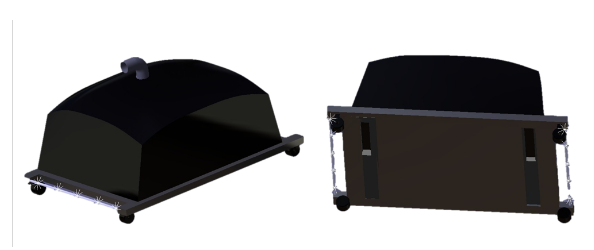
\includegraphics[width=0.8\textwidth]{figures/croqui-design-cpr.png}
    \caption{Croqui com o design do Clean Pool Robot, vista frontal e inferior.}
    \label{fig:croqui-design-cpr}
  \end{figure}
  \FloatBarrier
\par
Por motivo de resistência ao movimento o formato do robô foi modificado para melhor aproveitamento das forças hidrodinâmica envolvidas, as alterações no desenho inicial foram feitas com a intenção de diminuir a força de arrasto, a estrutura conta agora com cantos e arestas arredondadas conforme a Figura acima.

O design mostrado acima é a segunda versão onde foi melhorado o posicionamento das escovas, onde elas ficam na extremidade do robô onde auxiliar no impacto (por mais que seja pequeno) do robô com a parede em funcionamento.

\section{Sistemas}
O Robô possui três principais sistemas para o seu funcionamento: o Sistema de Automação, composto pelos sensores e programações lógicas de acionamento, Sistema de Locomoção, formado pelo conjunto das rodas, bomba e motores, e o Sistema de Limpeza, com os filtros e rolos de limpeza. O esquema abaixo mostra os três sistemas e a relação entre eles.
\par
  \begin{figure}[h]
    \centering
    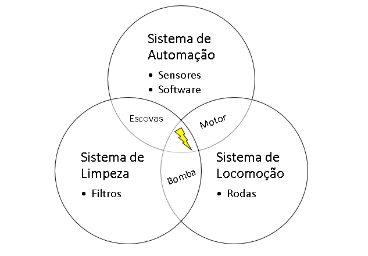
\includegraphics[width=0.8\textwidth]{figures/main-system-project.png}
    \caption{Três principais sistemas do Robô: Automação, Limpeza e Locomoção.}
    \label{fig:main-system-project}
  \end{figure}
  \FloatBarrier
\par

\section{Indicadores}
Como citado anteriormente o ciclo de limpeza é de 5h e possui uma taxa de filtragem de 2500 LPH (precisa colocar um texto explicando o pq desses indicadores).

\section{Custos}
No desenvolvimento do Clean Pool Robot foram gastos até o momento os valores apresentados na tabela abaixo. Considerando um lucro de 10\% sob cada peça, o custo estimado para a Venda do Robô é de R\$ 6.500, estando comercialmente competitivo.
\begin{table}[h]
\centering
\caption{My caption}
\label{my-label}
\begin{tabular}{@{}cc@{}}
Carga horaria máxima                      & 90 h         \\
Valor da Hora (Valor da Capes – Graduado) & R\$ 24, 44   \\
Pessoas no desenvolvimento do produto     & 12           \\
Hora por mês                              & 20           \\
Preço total da mão de obra                & R\$ 5.866,67 \\
Material                                  & R\$ 1.349,50 \\
Lucro                                     & 10\%         \\ \midrule
Valor total para Venda (sem impostos)     & R\$ 6.494,55
\end{tabular}
\end{table}

Uma pesquisa realizada apresentou o custo dos principais concorrentes do Clean Pool Robot que está entre R\$ 2.000,00 e R\$ 16.000,00, assim o valor de mercado está dentro da classe dos produtos mais baratos.

\chapter{Sistemas do Robô}
\section{O Sistema de Locomoção}
\subsection{Duto de Propulsão}
A água que é ejetada do sistema de filtragem é devolvida para a piscina já filtrada, auxiliando assim a limpeza geral de todo o volume em que o robô esta submerso. A água filtrada é direcionada para uma saída que se localiza na parte superior do produto. O duto de saída será um bocal direcionável localizado na parte superior do robô responsável por sua locomoção. Esse bocal irá se mover nas 4 direções principais, isto é, nos ângulos de 0, 90, 180 e 270 graus, proporcionando ao robô a locomoção necessária para o cumprimento da rota de limpeza.

O duto de propulsão terá diametro de 1” (25,4mm). Acoplado a ele está o propulsor auxiliar que permitirá a movimentação do robô com a velocidade desejada. O duto de propulsão foi construido de forma que a agua mude de direção sem que haja vazamentos e que o servo responsavel pela rotação não entre em contato com a água.

\subsection{As Rodas}
O aparelho contará com quatro rodas. Elas se assemelham as usadas em carrinhos de supermercado, com liberdade de 360 graus em relação ao eixo x e y.
\par
  \begin{figure}[h]
    \centering
    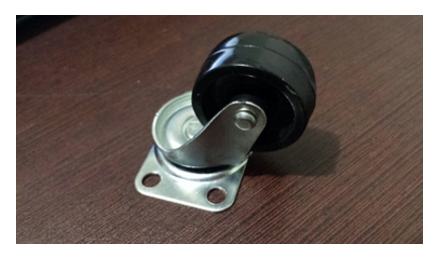
\includegraphics[width=0.6\textwidth]{figures/wheel-market.png}
    \caption{Rodas utilizadas para a locomoção do robô.}
    \label{fig:wheel-market}
  \end{figure}
  \FloatBarrier
\par
As rodas serão fixadas na placa da base do robô e estarão localizadas nos cantos da base do robô e direcionarão o seu movimento de acordo com a direção do jato de água oriundo do bocal, conforme a figura abaixo:
\par
  \begin{figure}[h]
    \centering
    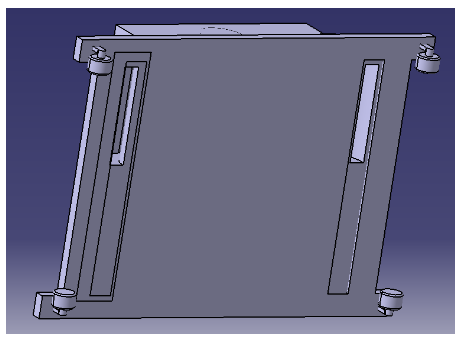
\includegraphics[width=0.8\textwidth]{figures/catia-base.png}
    \caption{Desenho da base do robô indicando as posições das rodas.}
    \label{fig:catia-base}
  \end{figure}
  \FloatBarrier
\par

\section{O Sistema de Limpeza}
\subsection{Os Filtros}
A filtragem irá garantir que a piscina estará limpa após o uso do Clean Pool Robot. O filtro será fundamental, pois ele será responsável pela remoção das partículas de sujeira que ficam decantadas no fundo da piscina. Primeiro a água será sugada para dentro do aparelho que passará por um depósito onde será feita a filtragem. Em seguida, a água filtrada retorna para piscina. Será realizado um sistema de dupla filtragem com dois tipos de elementos filtrantes: um de malha de alumínio, elemento secundário, para evitar que folhas e objetos de maior tamanho entrem no filtro principal que será responsável por filtrar o particulado e detritos da água.

Será usada uma malha de alumínio para a realização de uma pré-filtragem, a qual impedirá que folhas, plásticos, cabelos, e outros materiais maiores entupam o filtro principal responsável por retirar impurezas menores da água. Essa malha é o que chamou-se de filtro secundário. O filtro principal será um elemento filtrante na forma cilíndrica comumente utilizado na filtragem de caixas d’águas. As imagens dos filtros a serem utilizados e as especificações técnicas do elemento filtrante principal constam a seguir. Juntamente com o sistema de filtragem existe o que chamamos de “caixa de sujeira”, nela a pedras, folhas, galhos e outros objetos que poderam entupir ou diminuir a vazão de filtragem serão armazenadas. Essa caixa deverá ser limpa sempre que o robô for retrado da água.
\begin{description}
\item[Malha de Alumínio:] A malha de alumínio é um material durável, altamente resistente água, não precisa de manutenção e nem de troca. Em caso de avaria na grade a substituição é simples e barata. A grade será localizada na entrada da caixa filtradora, no duto de acesso na base do robô, conforme imagem abaixo.
\par
  \begin{figure}[h]
    \centering
    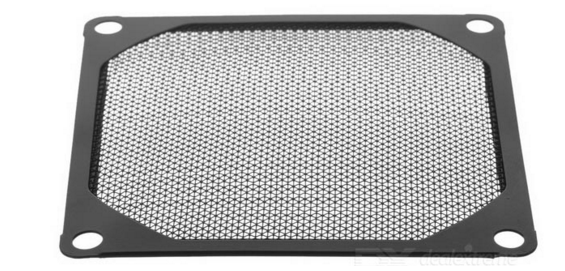
\includegraphics[width=0.8\textwidth]{figures/mesh-aluminium.png}
    \caption{Modelo de malha de alumínio utilizada como filtro secundário.}
    \label{fig:mesh-aluminium}
  \end{figure}
  \FloatBarrier
\par
\item[Elemento Filtrante:] as seguintes características são requeridas.

\begin{itemize}
\item Temperatura de operação: 5ºC mín. a 50ºC máx.
\item Vazão: 4.200 litros/hora
\item Grau de filtração: 50 micra (um grão de areia tem entre 200 a 500 micra)
\item Peso bruto: 448g
\item Peso líquido: 337g
\end{itemize}
Para se garantir a qualidade da água filtrada é indicado pelo fabricante a substituição dos elementos filtrantes Poly Flow a cada 6 meses ou quando for observada a redução do fluxo da água. O elemento filtrante é descartável, não necessita retrolavagem. A manutenção periódica do elemento é aconselhável. Para isso, utilize apenas água e uma escova macia.

Dimensões: Altura: 254mm; Diâmetro externo: 116mm; Diâmetro interno: 26mm.
\par
  \begin{figure}[h]
    \centering
    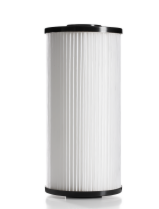
\includegraphics[width=0.5\textwidth]{figures/filter.png}
    \caption{Elemento Filtrante}
    \label{fig:filter}
  \end{figure}
  \FloatBarrier
\par
\end{description}
\subsection{O Dimensionamento dos Filtros}
Os filtros foram dimensionados, ou escolhidos, a partir dos pré-requisitos do projeto, isto é, velocidade, limpeza, area de atuação. Após a analise do que deveria ser filtrado e das possiveis fontes de entupimento do sistema de filtragem, dividiu-se o sistema em 3 áreas: caixa de sujeira; filtro secundario; filtro principal.

\subsection{Os Rolos de Limpeza}
Das principais sujeitas depositadas no fundo de piscinas pode-se listar: folhas e pequenos gravetos de arvores presentes nos arredores, além do acúmulo de algas, fungos e bactérias no fundo. Como solução para a limpeza destas sujeiras a utilização de peças com superficies mais macias ajudam a desgrudar do fundo as impurezas, independente de qual for o revestimento da piscina, se ele for azulejo, vinil, fibra ou pintura.(7)

Os rolos de limpeza estão localizados na parte frontal e traseira do robô, e  terão duas funções: a principal é auxiliar na remoção das impurezas do fundo da piscina, e a função secundária se dá no auxilio a sustentação do robô. 

Para o processo principal, a remoção das pequenas partículas depositadas no fundo da piscina, o rolo irá deslizar sob a superfície, sem que seja produzido muito atrito, para que não altere a velocidade total do robo e não danifique a superfície. Assim o material do rolo deve ser macio, leve e ao mesmo tempo resistente a água.

Para o processo secundário, de auxilio a sustentaçao do robô os rolos devem tem o seu raio na distância do fundo da piscina até a estrada de sucção, ou seja, a altura das rodas, pois assim o robô ficará nivelado e ao mesmo tempo com apoio na frente, atrás e no centro. Para esse requisito, o atendimento do design proposto, os rolos deverão ter, cada um deles, 300 mm de comprimento, 60 mm de diâmetro total e um eixo central com 30 mm de diâmetro, no qual será encaixado os eixos de rotação para os motores.

Definiu-se primeiramente utilizar escovas de formato cilíndrico e de Nylon, afim de que á medida que as rodas do robô se movem, as escovas também possam acompanhar o movimento sem maiores problemas. Porém a dificuldade em encontrar fabricantes e modelos em Brasilia e devido também ao elevado custo decidiu-se pela fabricação das escovas. Para a fabricação usou-se um tubo 50 mm de pvc e um revestimento de polimero, a fibra de vinil. 

A utlização de um polímero possui várias vantagens, tais como: baixa densidade, alta resistência à corrosão, baixo custo de aquisição, coeficiente de atrito baixo e grande flexibilidade. O baixo custo e densidade foram os principais motivos para a realização da troca.
\par
  \begin{figure}[h]
    \centering
    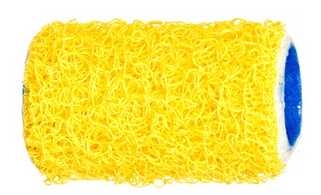
\includegraphics[width=0.5\textwidth]{figures/brush-vinil.png}
    \caption{Rolo de fibra de vinil.}
    \label{fig:brush-vinil}
  \end{figure}
  \FloatBarrier
\par

\section{Os Motores}
Serão utilizados dois motores elétricos para rotacionar os rolos de limpeza. A transmissão do torque para os rolos será por engrenagens. O modelo de motor a ser usado é o: Micro Motor DC 12V 18200RPM 390.40Gf.cm que possui as seguintes especificações:

Especificações técnicas do produto:
\begin{itemize}
\item Corrente: 1350,00 mA;
\item Potência: 6,40 W;
\item Tensão Nominal: 12,00 V;
\item Tensão Operacional: 6V ~ 18V;
\item Torque: 390,40 Gf.cm;
\item Velocidade: 18200 RPM;
\item Peso: 213g.
\end{itemize}

Especificações técnicas de máximo rendimento:
\begin{itemize}
\item Rotação: 15700rpm;
\item Corrente: 6.8A;
\item Torque 390gf.cm;
\item Potência: 6.4w;
\item Rendimento: 77.5%;
\item Torque de Partida: 1.3kgf.cm.
\end{itemize}

\subsection{O Dimensionamento}
Para a escolha dos motores foi utilizado 2 critérios: rotação das escovas e a massa das mesmas. O motor deverá ser capaz de rotacionar as escovas entre 2000 e 3000rpm e considerando que elas tem massa igual a 450g ter torque suficiente para realizar o giro.

\section{A Bomba}
A bomba participa dos dois sistemas referênciados acima, sistema de propulsão e limpeza. O processo de aspiração da piscina feito pelo robô será uma das principais tarefas executadas pela bomba de sucção, bem como também o processo de movimentação do robô embaixo d’água. Para isso, é importante que a bomba seja  forte o suficiente para sugar e gerar movimentação por meio do fluxo de saída da bomba. A sucção será conectada diretamente ao reservatório onde acontecerá a filtragem da água. É importante ressaltar que as únicas funções da bomba neste projeto são apenas filtrar e movimentar o robô através do empuxo gerado.

A análise do dimensionamento adequado para a bomba será feito a partir de sua vazão nominal. Para isto, tem-se por especificações primárias bombas que ofereçam vazões altas e que trabalhem em uma profundidade máxima de 3 metros.

\subsection{O Dimensionamento}
Para que pudesse definir qual bomba adquirir foi necessário realizar o dimensionamento da mesma, afim de que a bomba pudesse realizar a sucção da água e a  propulsão do robô abaixo d’água. Para isso, é necessário utilizar métodos que descrevem os cálculos que regem o movimento. Segundo
\citeonline{ise2000}, quando um veículo submersível se movimenta com velocidade constante,
a propulsão gerada pelos propulsores se iguala à força de arrasto produzida. A
força de arrasto será obtida a partir da soma da força de arrasto devido a 
movimentação do veículo mais a força de arrasto devido o cabo de alimentação.
\begin{displaymath}
  Fp = Fa = Fv + Fc = \frac{1}{2}\rho V^{2}_{v}Cd_{v} + \frac{1}{2}\rho V^{2}_{c}Cd_{c}
\end{displaymath}
Onde $Fp$ e $Fa$ referem-se à força de propulsiva e força de arrasto total
respectivamente; $Fv$ e $Fc$ são as forças de arrasto devido ao veiculo e ao cabo de
alimentação; $\rho$ é a densidade do fluido, $V_{v}$ e $V_{c}$ velocidades do
veículo e do cabo e por fim, $Cd_{v}$ e $Cd_{c}$ representam os coeficientes
de arrasto.
\par
A potência necessária para a bomba pode ser obtida em função da força propulsiva
e da velocidade do veiculo.
\begin{displaymath}
  P = Fp\frac{d}{t}
\end{displaymath}
Onde $d$ é a distancia percorrida, $t$ o tempo e $P$ a potência desejada.
\par
Os coeficientes de arrasto são medidos experimentalmente, para fluidos como
ar podem ser encontrados tabelados em função da velocidade do veiculo em relação
à velocidade do som nas condições do ambiente em questão (número de \textit{Mach}), uma
vez que este pode sofrer alterações devido a temperatura envolvida, meio de
propagação etc. Quando o veículo estudado se movimento em fluido líquido como a
água por exemplo, o coeficiente de arrasto deve ser medido em função do número
de Reynolds \cite{eng2008}, que por sua vez é calculado pela equação abaixo.
\begin{displaymath}
  Re = \frac{VD}{\upsilon}
\end{displaymath}
Onde $V$ equivale a velocidade do veículo, $D$ o diâmetro e $\upsilon$ a viscosidade
cinemática do fluido.
\par
\begin{figure}[h]
  \centering
  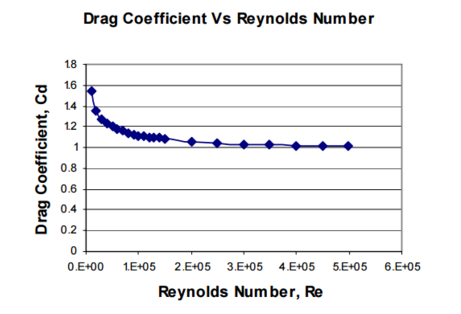
\includegraphics[width=0.9\textwidth]{figures/graphic-reynolds.png}
  \caption{Coeficiente de arrasto em função do número de Reynolds \cite{eng2008}}
  \label{fig:graphic-reynolds}
\end{figure}
\FloatBarrier
\par
[APLICANDO A EQ 1.......]

    \subsection{A Escolha da Bomba}
  \section{A Fonte de Alimentação}
    \subsection{O Dimensionamento}
    \subsection{Fonte Chaveada}
  \section{Vedação}
    \subsection{O Persilox}
  \section{A Mente do Robô (Eletrônica e Software)}
    \subsection{Central de Processamentos de Dados}
      \subsubsection{Os Requisitos}
      \subsubsection{Raspberry PI 2 B}
      \subsubsection{Arduino}
    \subsection{O Sistema de Controle de Tensão}
      \subsubsection{Os Requisistos/Dimensionamento}
      \subsubsection{GPIO - \textit{Generic Ports Input/Output}}
      \subsubsection{\textit{Driver} GPIO}
    \subsection{O Sistema de Sensoriamento}
      \subsubsection{Os Requisitos/Dimensionamento}
      \subsubsection{Os Sensores}
    \subsection{O Sistema de Rotação do Robô}
      \subsubsection{Os Requisitos/Dimensionamento}
      \subsubsection{Servo Motor}
    \subsection{Circuito Desenvolvido}
      \subsubsection{Diagrama do Circuito}
      \subsubsection{Pinagem}
    \subsection{Programação e Arquitetura de Software}
      \subsubsection{\textit{Middleware}}
      \subsubsection{Camada de Serviços}
        \subsubsubsection{Os Requisitos}
        \subsubsubsection{Serviço de Comunicação (I/O)}
        \subsubsubsection{Serviço de Concorrência}
      \subsubsection{Camada de Aplicação}
  
\chapter{Montagem do Robô}
  \section{Modelagem da Base do Robô}
  \section{Construção dos Rolos de Limpeza}

\chapter{Testes do \textit{Clean Pool Robot}}
  \section{Teste de Vedação - Persilox}
  \section{Testes do Protótipo}
  
\chapter{Resultados Parciais}
  














%O \textit{Clean Pool Robot} é um robô de aspiração de fundos de piscinas. O
%mecanismo do mesmo será composto por dois métodos para que o fundo da piscina
%possa ser aspirado: o primeiro baseia-se na escovação do chão e o segundo a
%sucção das impurezas desprendidas do piso da piscina.
%\par
%O primeiro método tem foco nas escovas que estão situadas na parte inferior
%do robô. As escovas realizam movimentos giratórios fazendo com que suas cerdas
%entrem em contato com o chão retirando  impurezas, como por exemplo: algas e
%grãos de terra.
%\par
%Após a escovação, é realizado outro método, a sucção das impurezas desprendidas
%do piso da piscina  além de outras impurezas que estiverem próximas à área de
%atuação do robô, por exemplo: pequenos ramos e folhas. Por meio de uma bomba, a
%água é sugada por uma abertura situada na parte inferior e passa por um saco onde
%as partículas de maiores dimensões ficam depositadas. Depois de passar pelo saco,
%a água passa por um filtro removível. As impurezas menores ficam retidas no filtro.
%Por meio de um sistema de expulsão de água, esta sairá a uma velocidade muito superior
%à velocidade de entrada no início do processo, ajudando também na movimentação do robô.
%\par
%Com o término da limpeza na piscina, haverá a necessidade dos filtros serem limpos
%para retirada das impurezas colhidas na aspiração da água. Assim, após cada utilização
%o usuário deverá limpar os filtros internos do \textit{Clean Pool Robot}.
%\par
%O produto desenvolvido será responsável apenas pela retirada da sujeira decantada
%no fundo da piscina, ou seja, o \textit{Clean Pool Robot} não limpará as paredes
%ou superfície da piscina. Além disso, as piscinas ideais para a operação do robô
%são as retangulares, sem inclinações e azulejadas. É ideal também que o robô seja
%lançado na piscina no meio da largura maior, evitando que o fio fique totalmente
%esticado quando o robô estiver na quina oposta do lançamento.
%\par
%Como diferencial, o \textit{Clean Pool Robot} será um produto nacional com custo
%mais acessível e que possui percurso não aleatório.
%\par
%O \textit{Clean Pool Robot} pode ser dividido em duas grandes partes, uma compondo a
%estrutura (apelidada de corpo) e o outro a parte lógica (apelidada de mente) do
%robô. Cada uma dessas será explicada posteriormente.
%
%\section{Percurso do Robô}
%O esquemático abaixo mostra uma ideia inicial de como o robô percorrerá a piscina
%a ser limpada.
%\par
%\begin{figure}[h]
%    \centering
%    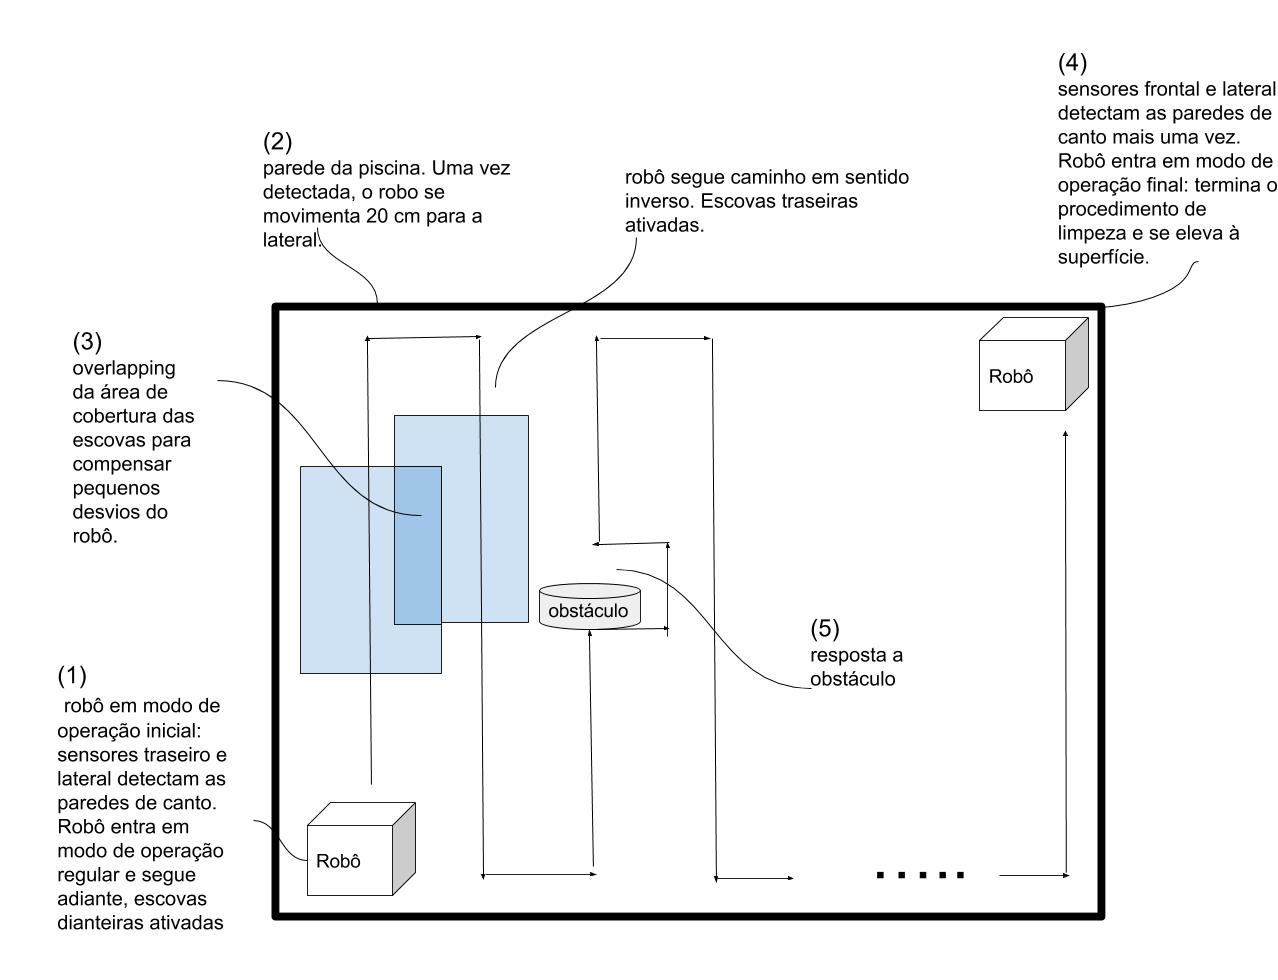
\includegraphics[width=\textwidth]{figures/schema-way-robot.jpg}
%    \caption{Demonstrativo do percurso de limpeza do robô (\textsf{Autoria do Autor})}
%    \label{fig:schema-way-robot}
%  \end{figure}
%\par
%O robô limpador foi projetado para ser capaz de percorrer toda a área da superfície
%inferior de piscinas retangulares e sem inclinação. A varredura é feita de forma
%totalmente autônoma pelo sistema, com a \textit{Raspberry pi} como unidade central de
%controle de todos elementos periféricos: sensores de distância, servo motores,
%sensores de pressão, etc. É necessário o usuário apenas posicionar o robô em
%uma das bordas da piscina e recolhê-lo quando o processo de limpeza estiver completo.
%\par
%Com o intuito de simplificar o sistema, optou-se por permitir ao robô mover-se apenas
%em duas direções, horizontal e vertical, em ambos os sentidos. Desta forma,
%baseando-se em projetos similares como o descrito na patente \textit{POOL CLEANER
%DIRECTIONAL CONTROL METHOD AND APPARATUS} \cite{porat2001}, o
%padrão ideal de varredura consiste em uma sequência de travessias longitudinais
%paralelas, partindo de uma borda da piscina à outra, como pode ser visto na Figura
%\ref{fig:schema-way-robot}.
%\par
%O robô inicia o processo de varredura assim que os sensores de distância,
%localizados em cada uma das laterais do robô, detectam que ele se encontra em
%uma das quinas da piscina (1).  O robô segue em linha reta em direção à
%próxima parede, com os motores das escovas ativados para fazer a limpeza do chão.
%Uma vez próximo à parede, robô então desloca-se para a direita cerca de 20
%centímetros e segue o percurso em linha reta, em sentido contrário (2). O deslocamento
%de 20 centímetros é tal que haja uma sobreposição das áreas varridas pelas escovas
%em ambos os sentidos percorridos (3), de forma a compensar qualquer desvio de
%rota não detectado pelo giroscópio. O robô retorna à parede inicial, desloca-se
%outros 20 centímetros para a direita  e segue mais uma vez em sentido oposto. Este
%procedimento se repete até que o robô chegue à parede direita da piscina (4). Na
%eventualidade do robô se encontrar, no meio do percurso,  com um obstáculo grande
%o bastante para ser detectado pelos sensores de distância, o robô deverá desviar
%do obstáculo e seguir sua rota original (5).
%
%\section{Modos de Operação}
%A movimentação do robô limpador é definida por quatro modos de operação distintos,
%referentes às quatro etapas de funcionamento: inicial, operação regular,
%resposta a obstáculo e final.
%\par
%Na etapa inicial, o robô deve ser capaz de submergir ao fundo da piscina e
%posicionar-se em um dos quatro vértices. Uma vez posicionado ele inicia o modo
%de operação regular e realiza o percurso de limpeza  explicado anteriormente.
%Terminado o percurso, o robô deve ser capaz de “emergir” à superfície para ser
%coletado pelo usuário. Caso o robô se depare com um obstáculo de grande porte
%em seu percurso, ele deve ser capaz de circundar o obstáculo e retornar ao modo de
%operação regular.
%
%\subsection{Modo de Operação Regular}
%O fluxograma a seguir define com mais detalhes as lógicas de funcionamento
%do robô limpador para o modo de operação regular, levando em conta todos os
%componentes eletrônicos envolvidos.
%\par
%\begin{figure}[h]
%  \centering
%  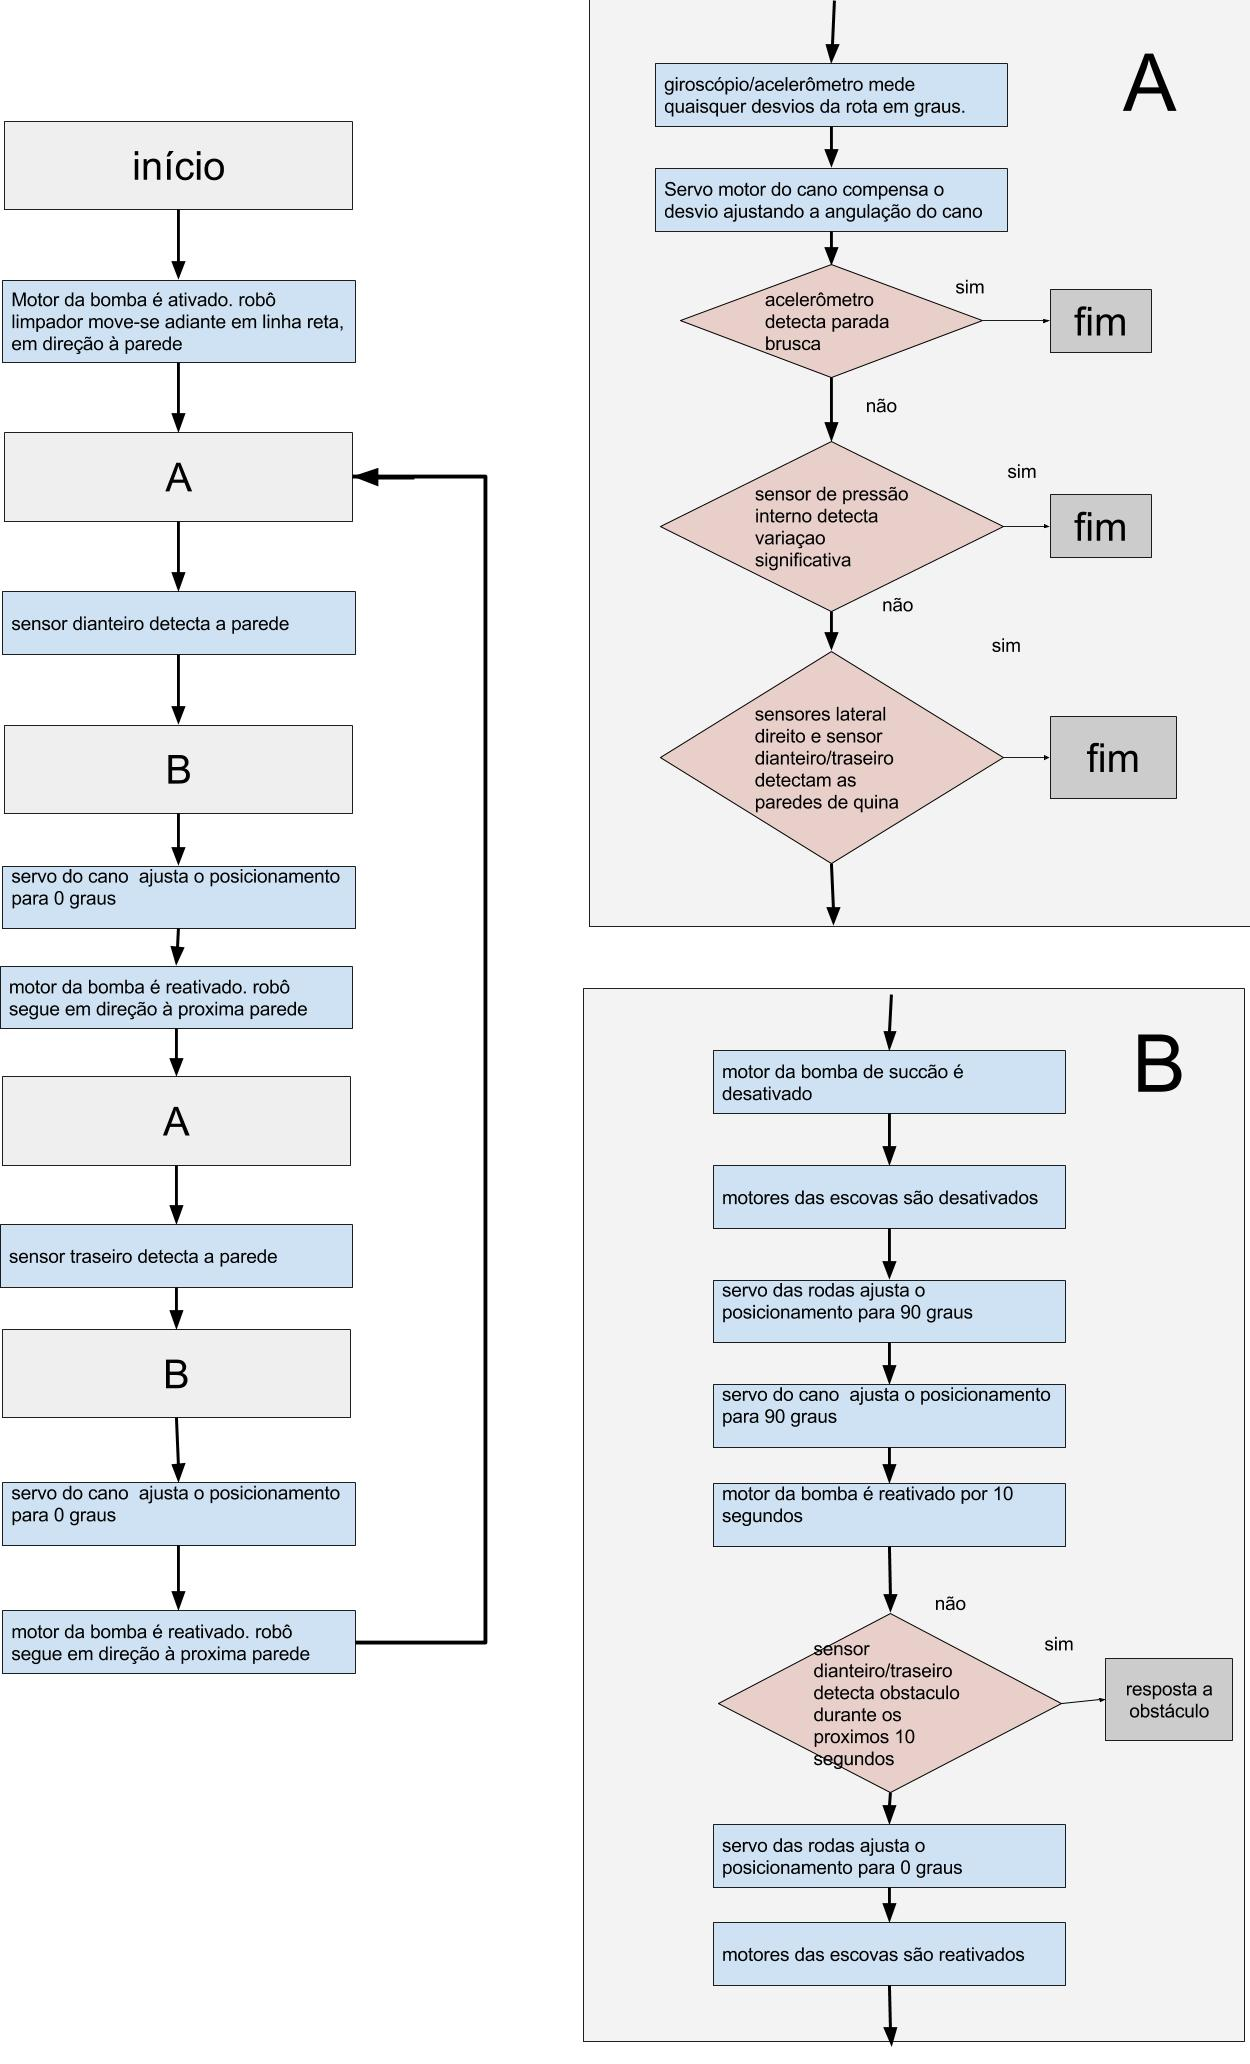
\includegraphics[width=0.8\textwidth]{figures/flow-regular-robot.jpg}
%  \caption{Modo de Operação Regular do \textit{Clean Pool Robot} (\textsf{Autoria do Autor})}
%  \label{fig:flow-regular-robot}
%\end{figure}
%\FloatBarrier
%
%\subsection{Resposta a Obstáculos}
%Foram definidos três casos de obstáculo que o robô poderá encontrar em seu percurso.
%
%\begin{description}
%\item[Caso 1:] \textit{Obstáculo pequeno capaz de ser sugado pela bomba e obstruir os
%filtros do limpador}. Neste caso, o sensor de pressão interna detecta qualquer
%variação de pressão na caixa do filtro.  A operação de limpeza é então abortada
%e o robô para e se “eleva à superfície” (modo de operação final).
%\item[Caso 2:] \textit{Obstáculo grande não detectado pelos sensores, resultando em
%colisão direta com obstáculo}. Neste caso, o acelerômetro detecta parada brusca
%do robô. A operação de limpeza é  também abortada e o robô para e se” eleva à
%superfície” (modo de operação final).
%\item[Caso 3:] \textit{Obstáculo grande e detectável pelos sensores de distância}. O
%robô não é capaz de imediatamente discernir a parede da piscina com o obstáculo
%e segue, a princípio, com seu procedimento como se o obstáculo fosse de fato parede.
%\end{description}
%\par
%O fluxograma a seguir detalha em alto nível de abstração as etapas que o sistema
%de controle devem seguir para circundar o obstáculo neste caso
%\par
%\begin{figure}[h]
%  \centering
%  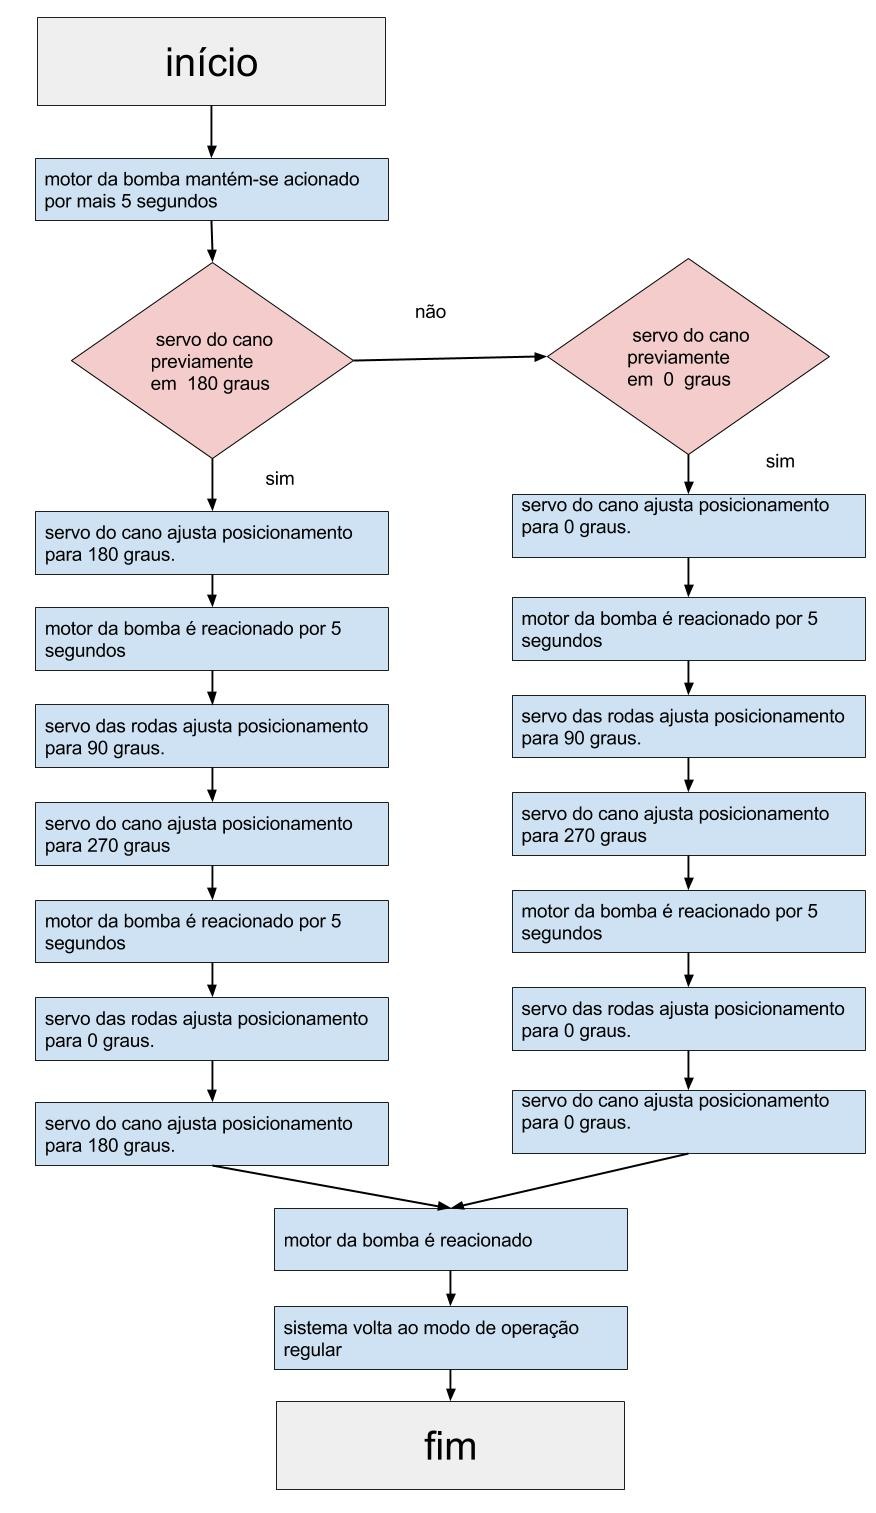
\includegraphics[width=0.7\textwidth]{figures/flow-robot-obstacle.jpg}
%  \caption{Modo de Operação Resposta a Obstáculos do \textit{Clean Pool Robot} (\textsf{Autoria do Autor})}
%  \label{fig:flow-obstacle-robot}
%\end{figure}
%\FloatBarrier
%
%\subsection{Modo de Operação Inicial e Final}
%Antes de começar a varredura da piscina, o robô deve primeiro posicionar-se
%perfeitamente em um dos 4 cantos da piscina. O fluxograma a seguir detalha
%as etapas do processo a partir do momento em que o robô chega ao fundo
%da piscina.
%\par
%\begin{figure}[h]
%  \centering
%  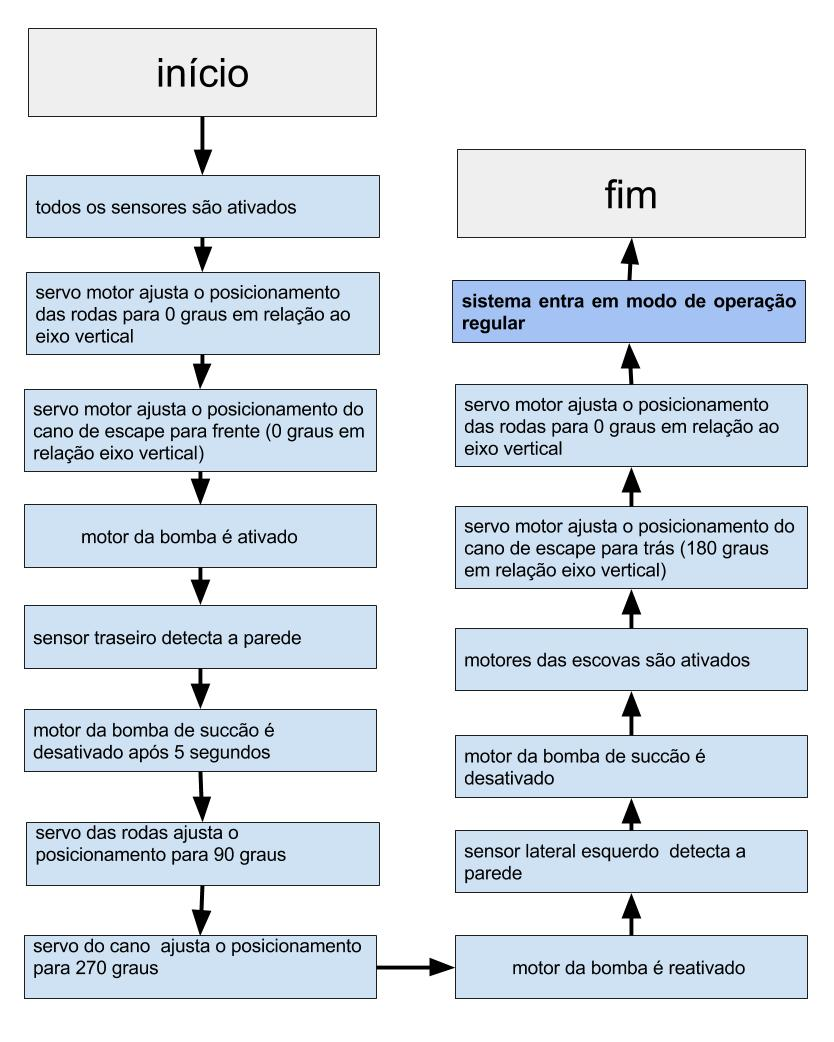
\includegraphics[width=0.8\textwidth]{figures/flow-initial-robot.jpg}
%  \caption{Modo de Operação Inicial e Final do \textit{Clean Pool Robot} (\textsf{Autoria do Autor})}
%  \label{fig:flow-initial-robot}
%\end{figure}
%\FloatBarrier
%
%\section{O Corpo do Robô (Aeroespacial, Automotiva e Energia)}
%A figura \ref{fig:initial_croqui} mostra a primeira modelagem do \textit{Clean Pool Robot}. O modelo
%apresenta uma bomba de sucção (1), uma caixa com os filtros para as impurezas
%(2), dois motores para a rotação das escovas (3), uma saída superior da água
%filtrada (4), quatro rodas próprias para rolagem em ambientes aquáticos (5),
%dois enrolamentos com escovas para soltura da sujeira do piso da piscina (6),
%duas entradas para sucção da água e impurezas do fundo da piscina (7), uma
%entrada da fonte de alimentação externa (8) e uma caixa com os circuitos
%eletrônicos do robô (9). Abaixo da figura \ref{fig:initial_croqui} estão detalhados as especificações
%de cada componente utilizado no Robô.
%\par
%\begin{figure}[h]
%  \centering
%  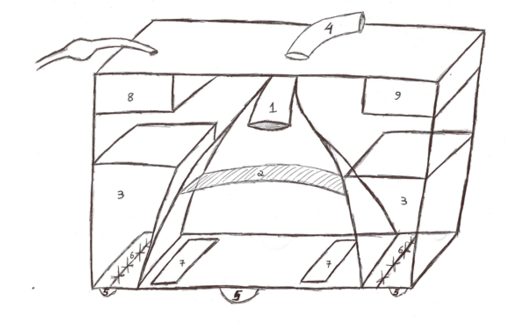
\includegraphics[width=0.8\textwidth]{figures/croqui.png}
%  \caption{ Croqui inicial do \textit{Clean Pool Robot} (\textsf{Autoria do Autor})}
%  \label{fig:initial_croqui}
%\end{figure}
%\FloatBarrier
%\par
%Por motivo de resistência ao movimento o formato do robô foi modificado para
%melhor aproveitamento das forças aerodinâmica envolvidas, as alterações no
%desenho inicial foram feitas com a intenção de diminuir a força de arrasto, a
%estrutura conta agora com cantos e arestas arredondadas conforme a Figura \ref{fig:better-croqui}.
%\par
%\begin{figure}[h]
%  \centering
%  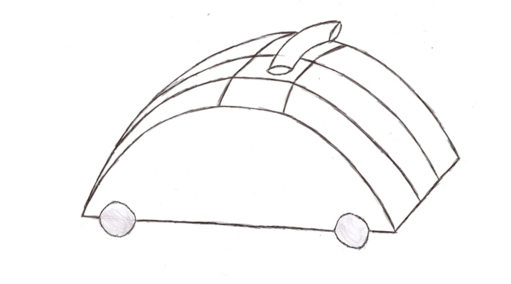
\includegraphics[width=0.8\textwidth]{figures/better-croqui.png}
%  \caption{ Croqui melhorado do \textit{Clean Pool Robot}(\textsf{Autoria do Autor})}
%  \label{fig:better-croqui}
%\end{figure}
%\FloatBarrier
%\par
%\begin{description}
%\item[Bomba:] O processo de aspiração da piscina feito pelo robô será uma das
%principais tarefas executadas pela bomba de sucção, bem como também o processo
%de movimentação do robô embaixo d’água. Para isso, é importante que a bomba
%seja forte o suficiente para sugar e gerar movimentação por meio
%do fluxo de saída da bomba. A sucção será conectada diretamente ao reservatório
%onde acontecerá a filtragem da água. É importante ressaltar que as únicas funções
%da bomba neste projeto são apenas filtrar e movimentar por empuxo.
%\par
%A análise do dimensionamento adequado para a bomba será feito a partir de sua vazão
%nominal. Para isto, tem-se por especificações primárias bombas que ofereçam vazões
%altas e que trabalhem em uma profundidade máxima de 3 metros. 
%\par
%Após o cálculo de sua velocidade de saída utilizando a sua vazão e área de jato,
%serão calculados o empuxo desenvolvido e sua respectiva pressão de saída. É importante
%salientar que a pressão de saída deverá ser sempre positiva e superior a pressão
%hidrostática a qual está submetido o bocal de propulsão.
%\par
%Ao longo de alguns estudos, observou-se que para o problema dado os modelos de bombas
%que melhor se enquadram são as moto bombas, uma vez que as mesmas possuem baixo peso e
%altas velocidades de saída, bem como altas vazões.
%\par
%O modelo parcialmente proposto será uma bomba do tipo Bilge , na qual tem as seguintes
%características:
%  \begin{itemize}
%  \item Peso: aproximadamente 3 kg;
%  \item Modelo: 500 GPH - com Tensão de trabalho 12 V DC - Amperagem de 1.9;
%  \item Formato: Cilíndrico alterável;
%  \item Área de operação entorno de até 3,7 metros.
%  \end{itemize}
%Observação: O formato da bomba poderá ser alterado de acordo com a eficiência
%esperada.
%\par
%\begin{figure}[h]
%  \centering
%  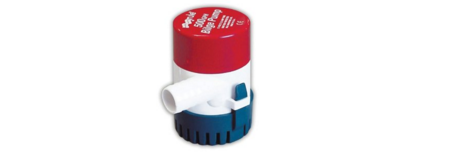
\includegraphics[width=0.9\textwidth]{figures/waterbomb.png}
%  \caption{Bomba proposta \cite{westmarine2016}}
%  \label{fig:waterbomb}
%\end{figure}
%\FloatBarrier
%\par
%\textit{Dimensionamento do Teste:} Diante de todo processo de dimensionamento
%e a propulsão do robô abaixo d’água, foi pensado em um teste para analisar se
%há coerência nos cálculos realizados. Sendo assim, o teste irá ser realizado
%com um uma estrutura móvel e uma bomba de aquário. É esperado, com isso, validar
%os cálculos realizados no que tange a movimentação da estrutura. Para isso, é
%necessário utilizar métodos que descrevem os cálculos que regem o movimento. Segundo
%\citeonline{ise2000}, quando um veículo submersível se movimenta com velocidade constante,
%a propulsão gerada pelos propulsores se iguala à força de arrasto produzida. A
%força de arrasto será obtida a partir da soma da força de arrasto devido a 
%movimentação do veículo mais a força de arrasto devido o cabo de alimentação.
%\begin{displaymath}
%  Fp = Fa = Fv + Fc = \frac{1}{2}\rho V^{2}_{v}Cd_{v} + \frac{1}{2}\rho V^{2}_{c}Cd_{c}
%\end{displaymath}
%Onde $Fp$ e $Fa$ referem-se à força de propulsiva e força de arrasto total
%respectivamente; $Fv$ e $Fc$ são as forças de arrasto devido ao veiculo e ao cabo de
%alimentação; $\rho$ é a densidade do fluido, $V_{v}$ e $V_{c}$ velocidades do
%veículo e do cabo e por fim, $Cd_{v}$ e $Cd_{c}$ representam os coeficientes
%de arrasto.
%\par
%A potência necessária para a bomba pode ser obtida em função da força propulsiva
%e da velocidade do veiculo.
%\begin{displaymath}
%  P = Fp\frac{d}{t}
%\end{displaymath}
%Onde $d$ é a distancia percorrida, $t$ o tempo e $P$ a potência desejada.
%\par
%Os coeficientes de arrasto são medidos experimentalmente, para fluidos como
%ar podem ser encontrados tabelados em função da velocidade do veiculo em relação
%à velocidade do som nas condições do ambiente em questão (número de \textit{Mach}), uma
%vez que este pode sofrer alterações devido a temperatura envolvida, meio de
%propagação etc. Quando o veículo estudado se movimento em fluido líquido como a
%água por exemplo, o coeficiente de arrasto deve ser medido em função do número
%de Reynolds \cite{eng2008}, que por sua vez é calculado pela equação abaixo.
%\begin{displaymath}
%  Re = \frac{VD}{\upsilon}
%\end{displaymath}
%Onde $V$ equivale a velocidade do veículo, $D$ o diâmetro e $\upsilon$ a viscosidade
%cinemática do fluido.
%\par
%\begin{figure}[h]
%  \centering
%  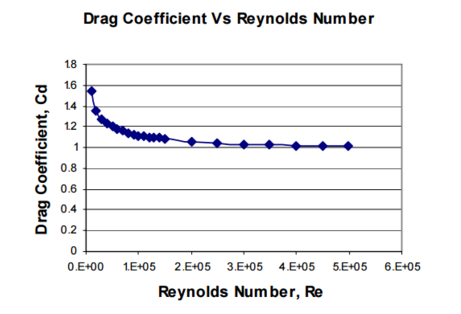
\includegraphics[width=0.9\textwidth]{figures/graphic-reynolds.png}
%  \caption{Coeficiente de arrasto em função do número de Reynolds \cite{eng2008}}
%  \label{fig:graphic-reynolds}
%\end{figure}
%\FloatBarrier
%\par
%Inicialmente a bomba utilizada será uma bomba de aquário, o que servirá de
%parâmetro para a determinação da bomba correta. Para isso, serão realizados
%testes com essa bomba para comprovação dos cálculos descritos acima.
%
%\item[Sistema Filtrador:] O sistema de filtragem irá garantir que a piscina
%estará limpa após o uso do \textit{Clean Pool Robot}. O filtro será fundamental,
%pois ele será responsável pela remoção das partículas de sujeira que ficam decantado
%no fundo da piscina. Primeiro a água será sugada para dentro do aparelho que passará por
%um depósito onde será feita a filtragem. Em seguida, a água filtrada retorna para
%piscina. Será realizado um sistema de dupla filtragem com dois tipos de elementos
%filtrantes, um de malha, secundário, para evitar que folhas e objetos de maior
%tamanho entrem no filtro principal que será responsável por filtrar o particulado
%e detritos da água.
%\begin{itemize}
%  \item Filtros: Usar-se-á uma malha de alumínio para a realização de uma
%  pré-filtragem, a qual impedirá que folhas, plásticos, cabelos, e outros
%  materiais maiores entupam o filtro principal responsável por retirar impurezas
%  menores da água. Essa malha é o que chamaremos de filtro secundário. O filtro
%  principal será um elemento filtrante na forma cilíndrica comumente utilizado
%  na filtragem de caixas d’águas. As imagens dos filtros a serem utilizados e as
%  especificações técnicas do elemento filtrante principal constam a seguir.
%  \item Malha de Alumínio: A malha de alumínio é um material durável, altamente
%  resistente a água, não precisa de manutenção e nem de troca. Em caso de avaria na
%  grade a substituição é simples e barata. A grade será localizada na entrada
%  da caixa filtradora, no duto de acesso na base do robô, conforme a Figura \ref{fig:eletric-motor}.
%  \par
%  \begin{figure}[h]
%    \centering
%    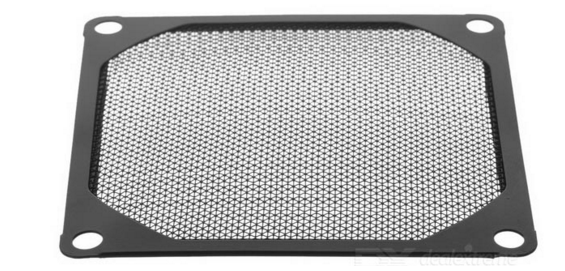
\includegraphics[width=0.9\textwidth]{figures/mesh-aluminium.png}
%    \caption{Modelo de malha de alumínio utilizada como filtro secundário. \cite{dx2016}}
%    \label{fig:mesh-aluminium}
%  \end{figure}
%  \FloatBarrier
%  \par
%  \item Elemento Filtrante:
%  \begin{itemize}
%    \item Temperatura de operação:  5ºC mín. a 50ºC máx;
%    \item Vazão: 4.200 litros/hora;
%    \item Grau de filtração: 50 micra (um grão de areia tem entre 200 a 500 micra);
%    \item Peso bruto:448 g;
%    \item Peso líquido: 337g.
%    \item Dimensões: Altura - 254mm; Diâmetro externo - 116mm; Diâmetro interno - 26mm.
%  \end{itemize}
%  Para se garantir a qualidade da água filtrada é indicado pelo fabricante a
%  substituição dos elementos filtrantes \textit{Poly Flow} a cada 6 meses ou quando
%  for observada a redução do fluxo da água. O elemento filtrante é descartável,
%  não necessita retrolavagem. A manutenção periódica do elemento é aconselhável.
%  Para isso, utilize apenas água e uma escova macia.
%  \par
%  \begin{figure}[h]
%    \centering
%    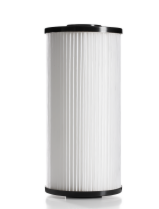
\includegraphics[width=0.2\textwidth]{figures/filter.png}
%    \caption{Elemento Filtrante - Refil POE IBBL 10'' \textit{Big Blue}}
%    \label{fig:filter}
%  \end{figure}
%  \FloatBarrier
%  \par
%  O elemento filtrante na forma cilíndrica, além de ser o mais encontrado
%  comercialmente, proporcionará ao CPR uma compactação dos dutos de filtragem
%  e uma melhor organização interna para alocação de seus componentes. O modelo
%  de filtro selecionado da \textit{Poly Flow} e similares é o que mais se encaixa as
%  necessidades de projeto e ao volume de trabalho da bomba a ser utilizada. Esses
%  modelos são comumente utilizados na filtragem de caixas d’águas, piscinas e banheiras.
%\end{itemize}
%\par
%O elemento filtrante na forma cilíndrica, além de ser o mais encontrado
%comercialmente, proporcionará ao CPR uma compactação dos dutos de filtragem e
%uma melhor organização interna para alocação de seus componentes. O modelo de
%filtro selecionado da Poly Flow e similares é o que mais se encaixa as
%necessidades de projeto e ao volume de trabalho da bomba a ser utilizada.
%Esses modelos são comumente utilizados na filtragem de caixas d’águas, piscinas
%e banheiras.
%
%\item[Motor:] Serão utilizados dois motores elétricos para rotacionar as escovas.
%a transmissão do torque para as escovas será por engrenagens, como ilustrado na
%Figura \ref{fig:eletric-motor}.
%\par
%\begin{figure}[h]
%  \centering
%  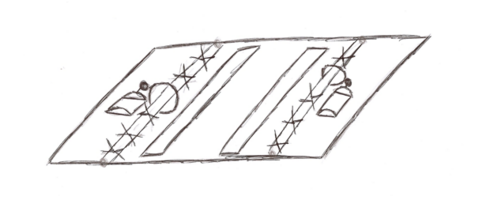
\includegraphics[width=0.7\textwidth]{figures/eletric-motor.png}
%  \caption{Atuação do motor elétrico (\textsf{Autoria do Autor})}
%  \label{fig:eletric-motor}
%\end{figure}
%\FloatBarrier
%
%\item[Saída Supeior de Água:] A água que é ejetada do sistema de filtragem é
%devolvida para a piscina já filtrada, auxiliando assim a limpeza geral de todo
%o volume em que o robô esta submerso. A água filtrada é direcionada para uma
%saída que se localiza na parte superior do produto. O duto de saída possui quatro
%aberturas imediatamente opostas que servem para direcionar o jato d’água,
%funcionando como o sistema de propulsão do produto. Quando uma das quatro aberturas
%estiverem sendo utilizadas para direcionar o jato, as outras três permanecem
%fechadas sendo utilizadas somente quando for necessário para a movimentação para a
%direção desejada. O duto de saída será um bocal direcionável localizado na
%parte superior do robô responsável por sua locomoção. Esse bocal irá se mover
%nas 4 direções principais, isto é, nos ângulos de 0, 90, 180 e 270 graus,
%proporcionando ao robô a locomoção necessária para o cumprimento da rota de limpeza.
%
%\item[Rodas:] O aparelho contará com dois tipos de rodas, a primeira em formato
%de esfera que será apenas para apoio. Foram utilizadas quatro rodas desse modelo.
%A segunda roda será para direcionar o aparelho no seu movimento, e será localizada
%no centro do robô, conforme imagem abaixo. A roda central será responsável pela
%alteração de direção do robo, sendo que apenas efetuará giros de  90º.
%\par
%\begin{figure}[h]
%  \centering
%  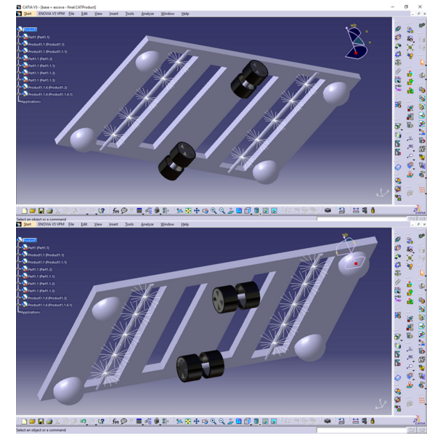
\includegraphics[width=0.6\textwidth]{figures/wheels.png}
%  \caption{Localização das rodas e rotação das rodas centrais (\textsf{Autoria do Autor})}
%  \label{fig:wheels}
%\end{figure}
%\FloatBarrier
%
%\item[Escovas:] Imaginou-se utilizar escovas de formato cilíndrico, afim de que
%à medida que as rodas do robô se movem, as escovas também possam acompanhar o
%movimento sem maiores problemas. As cerdas da escova devem possuir elevada
%resistência à tração, resistência à fadiga, baixo coeficiente de atrito e boa
%resistência térmica. Dessa forma como material para as cerdas sugere-se o
%\textit{Nylon} \cite{santos2010}.
%\par
%\begin{figure}[h]
%  \centering
%  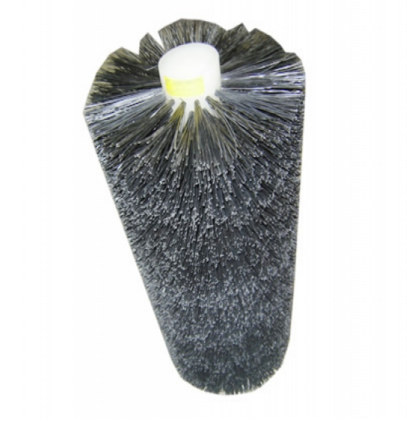
\includegraphics[width=0.4\textwidth]{figures/brush.png}
%  \caption{Modelo de escova sugerido para a limpeza da piscina \cite{santaclara2016}}
%  \label{fig:brush}
%\end{figure}
%\FloatBarrier
%A localização das escovas está ilustrada na figura \ref{fig:brush-local}, feita no software
%\textsf{CAD Catia V5 R19}. Serão utilizadas duas escovas movidas por motores elétricos,
%que farão a limpeza do chão.
%\par
%\begin{figure}[h]
%  \centering
%  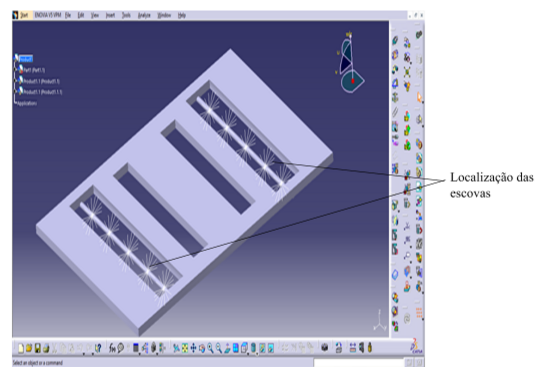
\includegraphics[width=0.8\textwidth]{figures/brush-local.png}
%  \caption{Localização das escovas no robô (\textsf{Autoria do Autor})}
%  \label{fig:brush-local}
%\end{figure}
%\FloatBarrier
%\par
%A movimentação das escovas será realizada por meio de engrenagens, como ilustrados
%na Figura \ref{fig:brush-system}. O motor elétrico fornecerá um torque e o sistema de
%engrenagem transmitirá para o eixo, fazendo com que as escovas rotacionem.
%\par
%\begin{figure}[h]
%  \centering
%  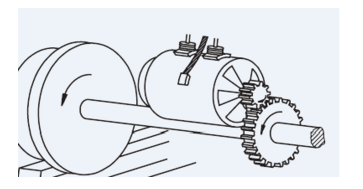
\includegraphics[width=0.8\textwidth]{figures/brush-system.png}
%  \caption{Sistema para movimentação das escovas.}
%  \label{fig:brush-system}
%\end{figure}
%\FloatBarrier
%
%\item[Entrada Inferior d'água:] A entrada ficará localizada logo após as
%escovas, como pode ser observado na figura \ref{fig:brush-local}.
%
%\item[Fonte de Alimentação Externa:] O \textit{Clean Pool Robot} é alimentado por
%uma fonte de energia que fica fora da água, através de um cabo de força. O Robô
%será alimentado pela tomada perto da piscina, em tensão de 220V (padrão Brasília).
%O cabo de alimentação terá um extensão que garante o deslocamento do robô por todas
%as extremidades da piscina durante a sua limpeza. Para o dimensionamento do
%comprimento do cabo foi calculado uma distância da tomada até a borda da piscina,
%somado ao maior comprimento possível para deslocamento do robô. Assim o comprimento
%do fio é dado por:
%\begin{displaymath}
%  L= d + D
%\end{displaymath}
%Onde o $L$ é o comprimento total do cabo de energia do robô, $d$ é a distância da
%tomada até a borda da piscina e $D$ é a distância a borda até o fundo da
%extremidade oposta a ela. Assim o cabo terá $L = 16,6 \approx 17m$. Considerando que
%a entrada do cabo na piscina se fará no ponto $P_ {ent}$, na metade da piscina,
%conforme a Figura \ref{fig:cable-desloc}.
%\par
%\begin{figure}[h]
%  \centering
%  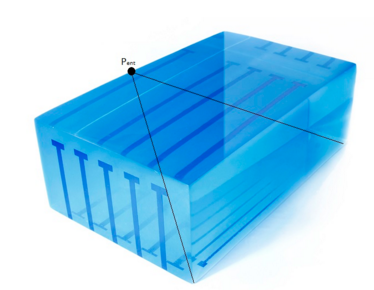
\includegraphics[width=0.8\textwidth]{figures/cable-desloc.png}
%  \caption{Deslocamento do cabo dentro da piscina \cite{assumpcao2014}}
%  \label{fig:cable-desloc}
%\end{figure}
%\FloatBarrier
%\par
%O cabo de energia possuirá uma boia presa ao logo da sua extensão para evitar
%enrolamento do cabo e possível ruptura do mesmo. O fio possuirá um revestimento
%de PVC impermeável e uma bitola estimada de 3,5 mm, para um potência consumida
%total de 350W.
%
%\item[Vedação:] É o processo que impede a passagem de líquidos, gases e
%sólidos particulados de um meio para outro. O material do vedador deve ser
%compatível com o produto para que não ocorra reações químicas causando vazamento
%e contaminação do produto.
%\par
%\begin{figure}[h]
%  \centering
%  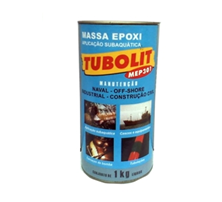
\includegraphics[width=0.4\textwidth]{figures/haha.png}
%  \caption{Massa Epoxi para vedação.}
%  \label{fig:haha}
%\end{figure}
%\FloatBarrier
%\par
%A massa Epoxi Tubolit Mep 301 funciona como proteção anti-corrosiva, proteção
%contra impactos, solda a frio, isolante elétrico, reparos em geral de furos,
%emendas e enchimentos, tanto dentro quanto fora d’água. Para aplicação
%subaquática: Manutenção Nava, Off-shore, Industrial, Construção Civil. Para
%revestimento e reparo em aço, concreto e outros materiais. Estruturas parcial
%ou totalmente submersas, oleodutos, hidroelétricas, plataforma de petróleo,
%estacas de concreto, tanques, reservatórios e caixas d'água.
%\end{description}
%
%\section{A Mente Do Robô (Eletrônica e Software)} \label{sec:mind-robot}
%A figura \ref{fig:schema-interactive-electro-soft} mostra a primeira esquematização
%da interação entre os componentes eletrônicos e os de \textit{software}. O modelo
%apresenta uma \textit{raspberry pi} (10), sensores de distância (11), pressão (12) e
%um acelerômetro/giroscópio (13), um conjunto de pinos (GPIO) (14), servo motor (15),
%relês (16), \textit{driver} da GPIO (17) e os serviços disponibilizados pelo \software  (18).
%Abaixo da figura \ref{fig:schema-interactive-electro-soft} estão detalhados as especificações
%de cada um desses componentes.
%\par
%\begin{figure}[h]
%  \centering
%  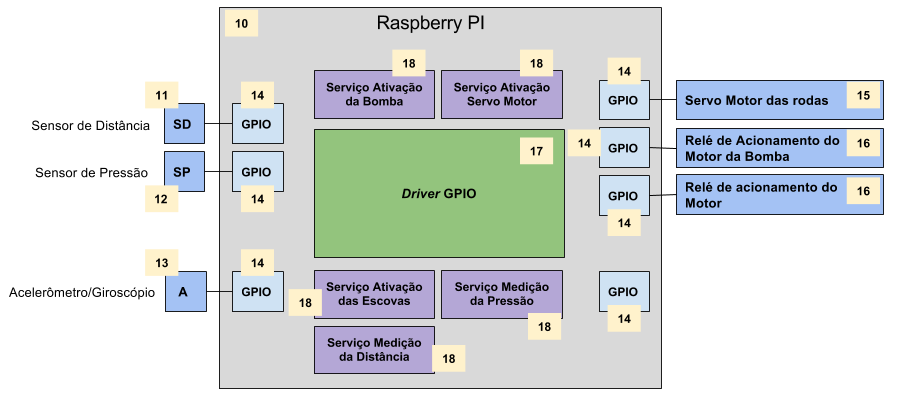
\includegraphics[width=\textwidth]{figures/schema-interactive-eletro-soft.png}
%  \caption{Esquemático da Interação entre Eletrônica e Software (\textsf{Autoria do Autor})}
%  \label{fig:schema-interactive-electro-soft}
%\end{figure}
%\FloatBarrier
%\par
%Os periféricos fornecerão dados que, por sua vez, serão passados ao \textit{driver} por
%meio de dispositivo de \hardware (GPIO).  O \textit{driver} será responsável por permitir
%a comunicação entre o \hardware e o \software que, na figura, é representado pelos
%serviços que deve fornecer ao sistema. Cada serviço tratará os dados de entrada
%conforme a especificidade solicitada e, em seguida, retorna uma saída para um
%atuador, por meio do \textit{driver}.
%\par
%\begin{description}
%\item[\rasp 2 B:] Com o objetivo de desenvolver um robô é necessário ter uma
%central de processamento de dados, a \rasp  foi escolhida pelo seu número de
%portas GPIO aonde pode ser desenvolvida a solução de sensores que existe
%para o problema. Além disso, seu suporte a sistema operacional, o que permite
%o uso de uma extensão maior de bibliotecas como a biblioteca \textit{pthread},
%e a possibilidade do uso de várias linguagens de programação também foram motivos
%para a escolha. \rasp é baseado em um \textit{SoC} - \textit{System on a Chip} -
%da \textit{Broadcom}, conhecido como \textsf{bcm2835}. Possui um processador
%de 700 MHz e memória RAM de 512 MB \cite{raspfoundation2014}.
%\par
%\begin{figure}[h]
%  \centering
%  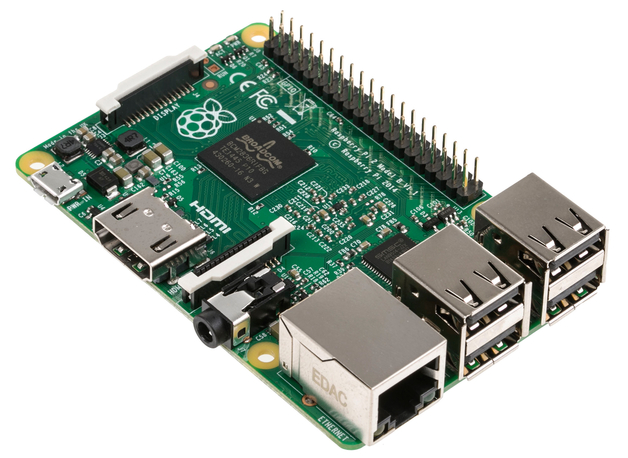
\includegraphics[width=0.8\textwidth]{figures/rpi2b.jpg}
%  \caption{\textit{Raspberry pi 2 B} \cite{raspfoundation2016}}
%  \label{fig:raspberry2b}
%\end{figure}
%\FloatBarrier
%
%\item[GPIO:] \textit{Generic Ports Input Output} são saídas e entradas de tensão.
%Elas servem para fazer a comunicação do processador com componentes externos,
%sensores e atuadores e outros tipos de componentes eletrônicos. Algumas dessas
%portas tem usos predefinidos pelo fabricante do \hardware como saídas de
%alimentação genérica, e terras, outros dos pinos são de uso genérico. A
%\textit{Raspberry pi} tem 40 pinos, aonde dessas 17 são para uso genérico.
%\par
%\begin{figure}[h]
%  \centering
%  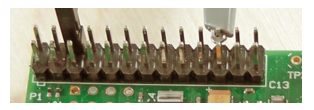
\includegraphics[width=0.6\textwidth]{figures/gpio.png}
%  \caption{GPIO \textit{Raspberry pi 2 B} \cite{raspfoundationgpio2016}}
%  \label{fig:raspberry2b}
%\end{figure}
%\FloatBarrier
%
%\item[Sensores de Distância:] serão utilizados sensores de distância com o
%intuito de permitir ao robô a identificação do espaço entre o robô e qualquer
%objeto à sua frente. Isso é importante para evitar colisões com as paredes da
%piscina e obstáculos a alturas que o sensor possa detectar. O sensor específico
%ainda não foi definido pois é necessário fazer teste com os propostos.
%
%\item[Sensores de Pressão:] O sensor de pressão proposta funciona com o
%princípios de materiais piezoelétricos, um liquido entra dentro da câmara
%e proporciona uma pressão nas paredes da câmara, esse pressão gera uma
%diferença de potencial no material. Com essa diferença de potencial é
%possível, usando um conversor AD (Analógico/Digital), saber a pressão dentro
%da câmara, e fora do robô.
%\par
%\begin{figure}[h]
%  \centering
%  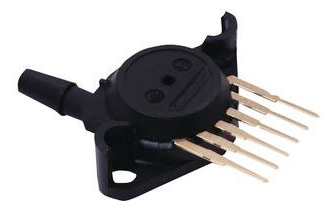
\includegraphics[width=0.6\textwidth]{figures/pressure-sensor.png}
%  \caption{Sensor de pressão MPX4250GP \cite{octopart2016}}
%  \label{fig:pressure-sensor}
%\end{figure}
%\FloatBarrier
%
%\item[Acelerômetro/Giroscópio:] Está sendo cogitado usar um acelerômetro
%para auxiliar o deslocamento em linha reta do robô e detectar choques com
%obstáculos grandes, quando ocorre um choque com um obstaculo grande não
%detectado pelo sensor de distancia a uma variação brusca na aceleração, com
%isso podemos tratar o obstaculo ou abortar o funcionamento do robô.
%\par
%No mesmo módulo se encontra um giroscópio, ele mede rotações no robô, caso
%seja identificado alguma rotação não pretendida pelo sistema podemos usar esse
%dado para corrigir a trajetória do mesmo. O componente eletrônico que tem os
%dois sensores se comunica através do protocolo I2C. Isso reduz o numero de
%pinos necessários pare ler os dados do sensor.
%\par
%\begin{figure}[h]
%  \centering
%  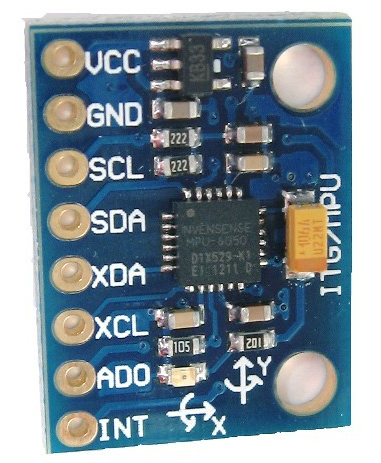
\includegraphics[width=0.5\textwidth]{figures/accelerometer.png}
%  \caption{Acelerômetro/Giroscópio MPU-6050 \cite{arduino2016}}
%  \label{fig:accelerometer}
%\end{figure}
%\FloatBarrier
%
%\item[Servo Motor:] Servos motores são utilizados para rotacionar um eixo até
%uma posição desejada. Esses motores são normalmente motores de alto torque.
%Dois servos (Micro Servo 9g e SG90 TowerPro) serão utilizados para rotacionar
%as rodas (5), o principal motivo de escolher esse modelo é ele ter torque
%suficiente para mover as mesmas e ter baixo custo, E para mover a saída de água
%(4) da bomba foi escolhido um servo motor (SM-S4306R) com maior liberdade de
%rotação (360º) e um maior torque.
%\begin{figure}[h]
%  \centering
%	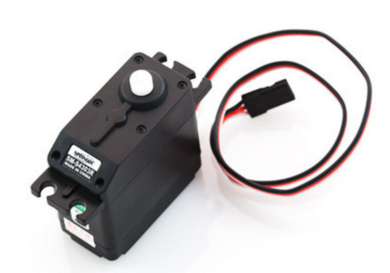
\includegraphics[height=5cm]{figures/servant-motor.png}
%	\quad
%	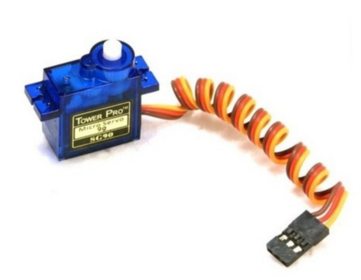
\includegraphics[height=5cm]{figures/micro-motor.png}
%  \caption{Servo Motores \cite{flipflop2013} e \cite{flipflop2016}, respectivamente}
%\end{figure}
%\FloatBarrier
%
%\item[Relé do Motor:] Os relés servem para fazer acionamento de circuitos
%de alta tensão usando como chaves circuitos de baixa tensão, além disso os
% relés servem para isolar os circuitos de baixa tensão dos de alta tensão.
% 
%\item[\textit{Driver} GPIO:] O driver é um \software que habilita a comunicação
%entre o \hardware e o \textit{software}. A partir do \textit{driver} é possível consumir os
%dados advindos dos componentes de \textit{hardware}, fazer o devido tratamento e, se
%necessário, enviar uma resposta \cite{windows2016}. Para o projeto foi
%identificada a biblioteca \textsf{bcm2835.h}, desenvolvida por Mike McCauley,
%que fará interface entre o \hardware e o \middleware, de forma que essa API
%terá o papel do \textit{driver}. Segundo \citeonline{mccauley2015}, a
%\textsf{bcm2835.h} fornece acesso à GPIO e demais funções da \textit{Broadcom}
%bcm2835, além de permitir acesso de leitura de sinais digitais, bem como de
%envio de sinais digitais, por meio da SPI ou I2C.
%\par
%A \textsf{bcm2835.h} é compatível com C++, bastando para o seu uso a adição do
%\textit{header} no código-fonte \cite{mccauley2015}. A documentação da
%\textsf{bcm2835.h} é extensa, o que provê suporte considerável para a equipe.
%Essa biblioteca é dividida em oito módulos:
%\begin{itemize}
%  \item Constantes para passagem: fornece \textsf{MACROs} para serem utilizadas
%  pela própria biblioteca ou programas externos que a estejam utilizando. Por
%  meio desse módulo pode-se, por exemplo, fazer a referência para um pino apenas
%  utilizando uma \textsf{MACRO}, sem preocupar-se como isso é referenciado
%  internamente \cite{mccauley2015}.
%  
%  \item Biblioteca de inicialização e gerenciamento: permite a inicialização da
%  \textit{broadcom} bcm2835 e seu gerenciamento \cite{mccauley2015}.
%  
%  \item Acesso de registro de baixo nível: normalmente o seu uso é desnecessário.
%  Fornece funções para o registro de baixo nível de informações \cite{mccauley2015}.
%  
%  \item  Acesso ao registro na GPIO: fornece funções que providenciam meios de ter
%  acesso à interface da GPIO. Por meio dessas funções pode-se fazer a leitura do
%  estado de cada pino, bem como ajustar o estado de saída para cada pino
%  \cite{mccauley2015}.
%  
%  \item Acesso à SPI: permite o uso da SPI0 (\textit{Serial Peripheral Interface})
%  para a comunicação com dispositivos externos SPI \cite{mccauley2015}.
%  
%  \item Acesso à I2C: fornece funções para uso da I2C (A \textit{Broadcom}
%  barramento de controle de série com o barramento/interface Philips I2C
%  versão 2.1 Janeiro de 2000) para comunicação com dispositivos externos
%  I2C \cite{mccauley2015}.
%  
%  \item Acesso ao Sistema de Tempo: permite acesso funções relativas ao
%  sistema contador de tempo \cite{mccauley2015}.
%  
%  \item Modularização de Largura de Pulso: permite o controle e a configuração
%  de dois canais indepentendes de PWM. Cada um dos canais pode ser conectado a
%  um subconjunto limitado de pinos da GPIO.
%\end{itemize}
%
%\item[\textit{Middleware} (Serviço):] é um \software que conecta outros componentes
%de \textit{software}. Uma camada de infraestrutura que viabiliza o desenvolvimento de
%aplicações voltadas ao negócio. Provê serviços que serão amplamente utilizados
%pela aplicação de negócio \cite{oracle2016}. O \middleware fornecerá serviços base para
%o robô, como ativação dos motores, escova e uso dos sensores. Inicialmente, imaginou-se
%a disponibilização de serviços para ativação de motores, bomba, escovas e leitura do
%\textit{output} dos sensores.
%\end{description}
%
%\subsection{Arquitetura de \textit{Software} e Programação}
%A Figura \ref{fig:schema-arch} mostra a abstração da arquitetura do sistema associado ao projeto.
%\par
%\begin{figure}[h]
%  \centering
%  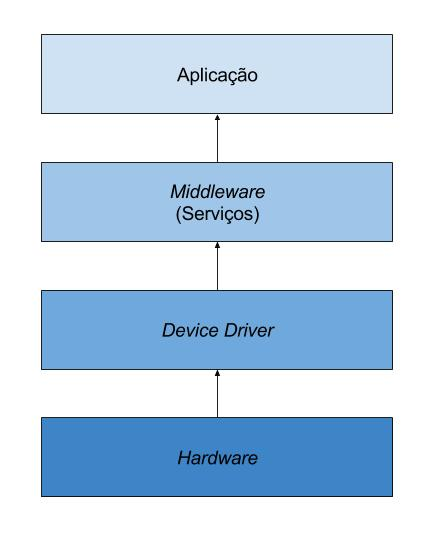
\includegraphics[width=0.4\textwidth]{figures/schema-arch.jpg}
%  \caption{Arquitetura em Camadas do \textit{Software} (\textsf{Autoria do Autor})}
%  \label{fig:schema-arch}
%\end{figure}
%\FloatBarrier
%\par
%O sistema segue uma arquitetura em camadas. A partir do \hardware os dados serão
%capturados. O \textit{driver} fará a ponte de comunicação entre o \hardware
%e o \textit{middleware}, permitindo que os dados possam ser trabalhados pela aplicação de
%negócio. A aplicação de negócio utilizará os serviços disponíveis pelo \textit{middleware},
%afim de tratar os dados recebidos e fornecer instruções ao robô. Uma visão
%ampliada da arquitetura está disponível na Figura \ref{fig:schema-layer-arch}.
%\par
%\begin{figure}[h]
%  \centering
%  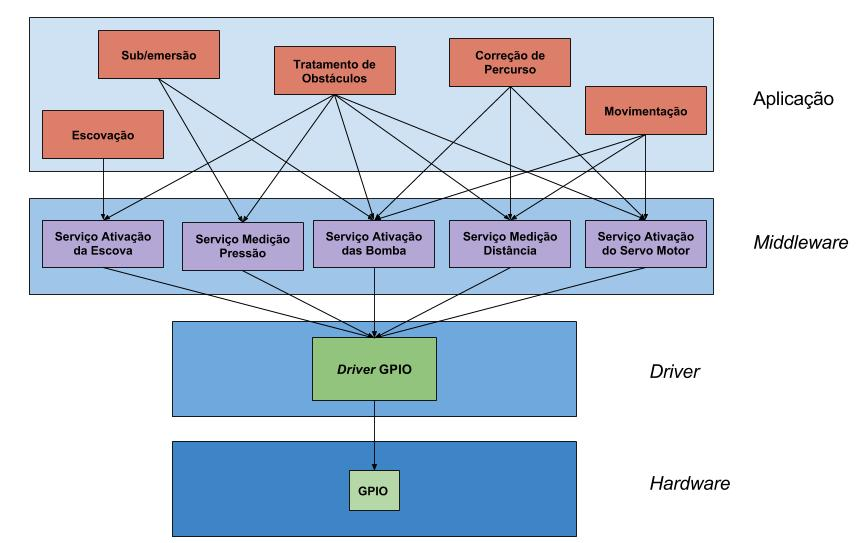
\includegraphics[width=0.9\textwidth]{figures/schema-layer-arch.jpg}
%  \caption{Detalhamento das Camadas e Interação dos componentes (\textsf{Autoria do Autor})}
%  \label{fig:schema-layer-arch}
%\end{figure}
%\FloatBarrier
%\par
%Foi selecionada a linguagem de programação \textsf{C++} para o desenvolvimento
%do projeto, por diversos aspectos associados a ela:
%\begin{itemize}
%  \item Linguagem multiparadigma: permite o uso de ferramentas relativas
%  ou paradigma estruturado, orientado a objetos e programação genérica. Essa
%  característica, segundo \citeonline{stroustrup2012}, criador da linguagem, apresenta
%  ao programador a possibilidade de utilizar as melhores características de
%  cada forma de programação.
%  
%  \item Linguagem de baixo nível: linguagem voltada a aplicações que exigem
%  a compreensão da arquitetura do computador.
%  
%  \item Biblioteca Padrão de \textit{Templates}: fornece diversas classes e
%  funções que facilitam a produção de \textit{software}, evitando retrabalho.
%\end{itemize}
%\par
%O desenvolvimento do \software será cooperativo e distribuído. Conforme descrito na
%seção \ref{sec:mind-robot}, a \rasp permite o uso de um sistema operacional. Para
%padronizar o desenvolvimento com o mesmo sistema operacional instalado na
%\textit{Raspberry pi}, usar-se-á a ferramenta de virtualização \textsf{Vagrant}.
%O \textsf{Vagrant} é uma ferramenta para a construção de ambientes de desenvolvimento
%focada num fluxo de trabalho simples e automação da configuração desse ambiente
%\cite{hashicorp2016}.
%\par
%O uso do \textsf{Vagrant} permitirá também que o ambiente de desenvolvimento de
%cada membro da equipe seja igual, com as mesmas bibliotecas instaladas e ferramentas.
%Essa padronização evitará dificuldades de compatibilidade entre o ambiente dos
%desenvolvedores e o instalado na \textit{Raspberry pi}.
%\par
%O Código \ref{vagrantfile} mostra as configurações da \textit{box} criada para o
%projeto:
%\par
%\begin{lstlisting}[language=Ruby, label=vagrantfile, caption=\textsf{Vagrantfile} inicial]
%Vagrant.configure(2) do |config|
%  config.vm.box = "debian/jessie64"
%
%  config.vm.provision "shell", path: "scripts/gpp.sh"
%  config.vm.provision "shell", path: "scripts/libraries.sh"
%end
%\end{lstlisting}
%\par
%Observa-se pelo Código \ref{vagrantfile} que as configurações foram divididas em
%dois \textit{scripts}, descritos nos Códigos \ref{gpp.sh} e \ref{libraries.sh}.
%\par
%\begin{lstlisting}[language=bash, label=gpp.sh, caption=\textsf{Script} para instalação
%de ferramentas de compilação]
%#!/usr/bin/env bash
%
%echo "Installing: ( 1 ) g++, ( 2 ) gcc and ( 3 ) make"
%
%echo "Install g++: starting"
%sudo apt-get install g++ -y
%echo "Install g++: DONE"
%
%echo "Install gcc: starting"
%sudo apt-get install gcc -y
%echo "Install gcc: DONE"
%
%echo "Install Make: starting"
%sudo apt-get install build-essential
%echo "Install Make: DONE"
%\end{lstlisting}
%\par
%\begin{lstlisting}[language=bash, label=libraries.sh, caption=\textsf{Script} para instalação
%de bibliotecas externas]
%#!/usr/bin/env bash
%
%echo "Installing: ( 1 ) bcm2835 and ( 2 ) boost-libraries"
%
%echo "Install bcm2835.h: starting"
%sudo wget http://www.airspayce.com/mikem/bcm2835/bcm2835-1.50.tar.gz
%tar zxvf bcm2835-1.50.tar.gz
%rm bcm2835-1.50.tar.gz
%cd bcm2835-1.50
%./configure
%make
%sudo make check
%sudo make install
%echo "Install bcm2835.h: DONE"
%
%echo "Updating: starting"
%sudo apt-get update
%echo "Updating: DONE"
%
%echo "Install boost-libraries: starting"
%sudo apt-get install libboost-all-dev -y
%echo "Install boost-libraries: DONE"
%\end{lstlisting}
%\par
%Será utilizado também uma ferramenta para o controle de versão do código. O
%\textsf{Git} foi selecionado para cumprir essa função, enquanto que o
%\textsf{GitHub} foi escolhido como repositório remoto. O controle de versão permite
%o gerenciamento das diversas versões de um determinado documento. É comum o
%seu uso no desenvolvimento de \textit{software}, o que fornece um controle do histórico
%de alterações, permitindo o resgate de versões antigas. Outra vantagem no uso desse
%tipo de sistema é a facilidade em trabalhar em equipe sobre os mesmos documentos,
%pois fornece ferramentas que minimizam problemas de conflito de alterações. A
%divisão do projeto em ramos de trabalho, permitindo o desenvolvimento paralelo
%de diferentes partes do \software pela equipe, também é uma vantagem no
%versionamento do código.